% \input utf8-t1
\documentclass[12pt,titlepage,a4paper]{extarticle}

% ------ PACKAGES ------

\usepackage[czech]{babel}
\usepackage[utf8]{inputenc}
\usepackage[paper=a4paper,top=2cm,left=3.5cm,right=2cm,bottom=2cm,includefoot]{geometry} % odsazení a velikosti stránek
\usepackage[bookmarksopen,bookmarks,pdfauthor={Josef Kolar},pdftitle={Souboje virtualnich robotu PYBOTS},pdfsubject={herni server PYBOTS pro programatory},pdfkeywords={python,game,programmers,flask,maze,bots}]{hyperref} % odkazy
\usepackage[titles]{tocloft} % pro stylování obsahu
\usepackage{listings} % výpisy zdrojových kódů
\usepackage{color} % barvy
\usepackage{xcolor} % vytváření barev
\usepackage{newverbs}
\usepackage{todonotes} % todo značky
\usepackage{graphicx} % načítání grefiky
\usepackage{float} % podpora pro figure s H pozicí
\usepackage{lipsum} % dummy text
\usepackage{svg} % inludesvg
\usepackage[tableposition=above]{caption} % vlastní styly pro caption
\usepackage{wrapfig} % figure v textu
\usepackage{titling} % theauthor, thetitle
\usepackage{fancyhdr} % zápatí, záhlaví
\usepackage{lastpage} % lastpage label
\usepackage{tabularx} % pro responzivni tabulky
\usepackage{array} % pro tabulkové zápis
\usepackage[verb]{collcell} % pro sloupce s makrem
\usepackage{bookmark} % nenutnost spouštět dvakrát pro korektní reference
\usepackage{pdfpages} % inlude pdf
\usepackage{titlesec} % \section na nové stránce
\usepackage{longtable} % tabulka přes více stránek
\usepackage{datetime} % pro formáty datumů
\usepackage{pdflscape} % pro jednu stránku na šířku

% ------ CONFIGURATION ------

% violet 3300CC
% red CC0011
\definecolor{codeprimary}{HTML}{3300CC}
\colorlet{keywordstyle}{codeprimary!50!black}

\definecolor{linkcolor}{HTML}{CC0011}
\colorlet{keywordstyle}{linkcolor}

% \colorlet{codeprimary}{blue!80!red}
\colorlet{lightgray}{gray!5}

\colorlet{jsonnumber}{blue}
\colorlet{jsonpunct}{red}
\colorlet{jsondelim}{codeprimary}

\definecolor{emptyfield}{HTML}{CCCCCC}
\definecolor{treasurefield}{HTML}{FFFF00}
\definecolor{botfield}{HTML}{FF4500}
\definecolor{blockfield}{HTML}{999999}
\definecolor{laserbatterybotfield}{HTML}{7D2A69}

\setlength{\cftbeforesecskip}{14pt}
\setlength{\cftbeforesubsecskip}{7pt}
\setlength{\cftbeforesubsubsecskip}{3.5pt}

% default width of svg
\setsvg{width=.5\textwidth}
\graphicspath{ {assets/} }

% reset ref section names
\def\sectionautorefname{}
\def\subsectionautorefname{}
\def\subsubsectionautorefname{}
\def\tableautorefname{}
\def\figureautorefname{}
\renewcommand\lstlistlistingname{Seznam zdrojových kódů}
\renewcommand\lstlistingname{Zdrojový kód}

\lhead{Praktická zkouška z~odborných předmětů - Souboje virtuálních robotů PYBOTS}
\chead{}
\rhead{}
\lfoot{}
\cfoot{}
\rfoot{Strana \thepage \hspace{1pt} z~\pageref*{LastPage}}
\addtolength{\headheight}{1.2pt}
\renewcommand{\headrulewidth}{2pt}
\renewcommand{\footrulewidth}{0pt}
\renewcommand{\arraystretch}{1.2}

\title{Souboje virtuálních robotů PYBOTS}
\author{Josef Kolář}
\date{\today}

% ------ CUSTOM COMMANDS ------

% \ic for inline code
\makeatletter
\newcommand\ic[1][green]{%
    \@testopt{\@ic{#1}}{-#1}% Handle second optional argument
}
\def\@ic#1[#2]{%
    \Collectverb{\@@ic{#1}{#2}}%
}
\def\@@ic#1#2#3{%
    \fcolorbox{white}{lightgray}{\lstinline[basicstyle=\ttfamily\color{codeprimary},breaklines=true]|#3|}%
}
\newcommand{\icmacro}[1]{\fcolorbox{white}{lightgray}{\lstinline[basicstyle=\ttfamily\color{codeprimary},breaklines=true]|#1|}}
\makeatother

% \lstnewenvironment{code}[3][]%
%   {\noindent%
%     \minipage{\linewidth}%
%     \lstset{#1,#2,#3}%
%   }{\endminipage}%

\lstnewenvironment{code}[1][]%
{\noindent\minipage{\linewidth}\lstset{frameround=fttf,#1}}%
{\endminipage}%

% ref as <number of section> <title of section>
\newcommand*{\fullref}[1]{\hyperref[{#1}]{\autoref*{#1} \nameref*{#1}}}

\newenvironment{bottompar}{\par\vspace*{\fill}}{\clearpage}

\newcolumntype{B}{>{\collectcell\icmacro}r<{\endcollectcell}}

% ------ LISTINGS SETUP ------

\lstset{
    language=Python,
    frameround=fttf,
    breaklines=true,
    keywordstyle=\color{keywordstyle}\ttfamily,
    basicstyle=\color{codeprimary},
    numberstyle=\color{black},
    backgroundcolor=\color{white},
    frame=single,
    tabsize=4,
    breaklines=true,
    captionpos=t,
    xleftmargin=\dimexpr\fboxsep+1pt\relax,
    xrightmargin=\fboxsep,
    numberstyle=\scriptsize,
    numbersep=7pt,
    numbers=left,
    showstringspaces=false,
    escapeinside={\#!}{\^^M},,
    belowcaptionskip=3pt,
    belowskip=3pt,
    aboveskip=0pt,
}

\DeclareCaptionFormat{listing}{%
	\colorlet{currentcolor}{.}%
	{\color{codeprimary}{\framebox[\textwidth+1pt]{\color{currentcolor}#1#2#3}}}%
}
\captionsetup[lstlisting]{format=listing, singlelinecheck=false}

\lstdefinelanguage{json}{
    basicstyle=\color{codeprimary},
    numberstyle=\scriptsize,
    numbersep=8pt,
    numbers=left,
    breaklines=true,
    frame=single,
    %backgroundcolor=\color{background},
    literate=
     *{0}{{{\color{jsonnumber}0}}}{1}
      {1}{{{\color{jsonnumber}1}}}{1}
      {2}{{{\color{jsonnumber}2}}}{1}
      {3}{{{\color{jsonnumber}3}}}{1}
      {4}{{{\color{jsonnumber}4}}}{1}
      {5}{{{\color{jsonnumber}5}}}{1}
      {6}{{{\color{jsonnumber}6}}}{1}
      {7}{{{\color{jsonnumber}7}}}{1}
      {8}{{{\color{jsonnumber}8}}}{1}
      {9}{{{\color{jsonnumber}9}}}{1}
      {:}{{{\color{jsonpunct}{:}}}}{1}
      {,}{{{\color{jsonpunct}{,}}}}{1}
      {\{}{{{\color{jsondelim}{\{}}}}{1}
      {\}}{{{\color{jsondelim}{\}}}}}{1}
      {[}{{{\color{jsondelim}{[}}}}{1}
      {]}{{{\color{jsondelim}{]}}}}{1},
}

% ------ HYPERREF SETUP ------
\hypersetup{
	colorlinks,
	linkcolor=linkcolor,
	citecolor=linkcolor,
	urlcolor=linkcolor,
  bookmarks,
  bookmarksopen,
  bookmarksdepth=2
}
\begin{document}
\pagestyle{fancy}

\begin{titlepage}
	\centering

	\begin{figure}[H]
		\centering
		\includesvg[width=.25\textwidth]{images/spseol-logo}
	\end{figure}

	{\LARGE \bfseries Vyšší odborná škola a Střední průmyslová škola elektrotechnická Olomouc Božetěchova 3}

	\vspace*{\fill}

	\fontsize{20pt}{30pt}{\bfseries PRAKTICKÁ ZKOUŠKA Z ODBORNÝCH PŘEDMĚTŮ\\\thetitle\\}

	\vfill

	{\LARGE \bfseries 2016 \hfill \theauthor}
\end{titlepage}
% \begin{titlepage}
  \begin{center}

  \textsc{\LARGE Vyšší odborná škola a Střední průmyslová škola elektrotechnická Olomouc}

  \begin{figure}[H]
    \centering
    \includesvg[width=.2\textwidth]{assets/spseol-logo}
  \end{figure}

  \textsc{\Large STŘEDOŠKOLSKÁ ODBORNÁ ČINNOST}\\[0.5cm]
  Obor 10. elektrotechnika, elektronika a telekomunikace\\[.2cm]
	
  \rule{\linewidth}{0.5mm} \\[.4\linewidth]
  
  {
    \huge \bfseries \thetitle
  }

  \rule{\linewidth}{0.5mm} \\[.4\linewidth]
  
  SDR RECEIVER FOR SW BAND\\
		
  \emph{Autor:} Josef \textsc{Kolář}
  
  \vfill

  {\large \today}

  \end{center}
\end{titlepage}


% \setcounter{page}{3}

\newenvironment{signaturedtext}{\large}{%
	\newline
    \begin{flushright}
		\begin{minipage}[H]{.5\textwidth}
			\begin{center}
				\dotfill\newline
				jméno a příjmení studenta
			\end{center}		
		\end{minipage}
	\end{flushright}
}

\clearpage
\thispagestyle{empty}

\begin{signaturedtext}
	Prohlašuji, že jsem praktickou zkoušku vypracoval samostatně a všechny prameny jsem uvedl v~seznamu referencí.
\end{signaturedtext}

\vspace*{\fill}

\begin{signaturedtext}
	Mé poděkování patří panu \emph{Ing. Marku Nožkovi} za vedení při této práci, nasměrování k~systému \textbf{\LaTeX} a neutuchající nadšení pro výuku, a mým spolužákům \emph{S. H. Nguenovi} a \emph{J. Hanákovi} za jejich návrhy na vylepšení této práce a použité jmenné konvence. 
\end{signaturedtext}
	
\vfill
	
\begin{signaturedtext}
	Prohlašuji, že nemám námitek proti půjčování nebo zveřejňování mé práce, nebo její části se souhlasem školy.
\end{signaturedtext}

\clearpage

% \begin{abstract}
% \lipsum[2]
% \end{abstract}

\newpage
\setcounter{page}{4}
\addtocontents{toc}{~\hfill\textbf{Strana}\par}
\addcontentsline{toc}{section}{Obsah}
{\large\tableofcontents}

\newpage
\addcontentsline{toc}{section}{Zadání}
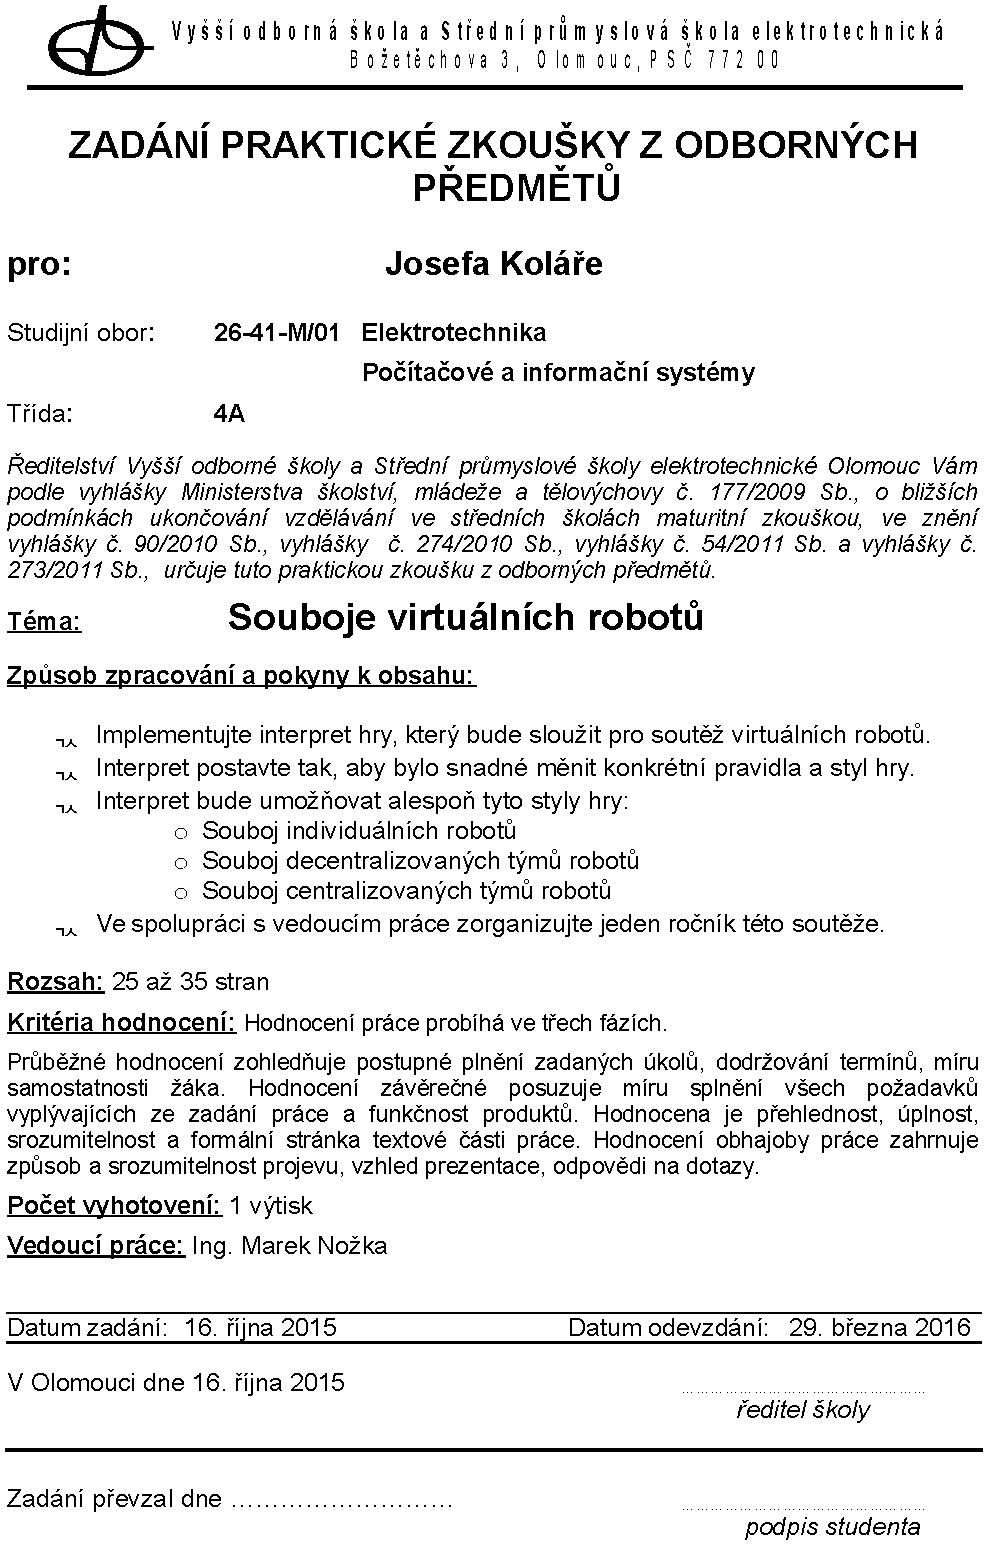
\includepdf[pages={1},width=\textwidth]{assets/zadani.pdf}

\newpage
\pagestyle{fancy}
\newcommand\sectionbreak{\clearpage}


\section{Teoretický úvod}

\subsection{Rozbor zadání}
\todo{rozbor jednotlivých bodů}
\subsection{Návrh architektury aplikace}

\subsubsection{Návrh interní struktury}

\textit{
	V této sekci se budu zabývat pouze teoretickým návrhem jednotlivých datových a řídící struktur. Popisu použitých algoritmů a jednotlivých implementačních rozhodnutí se budu věnovat v sekci\fullref{sec:implementation}.
}

O interní reprezentaci jedné instance hry se stará třída \ic|Game|, která je zodpovědná za striktní přístup klienta do mapy. Zpracovává jednotlivé herní akce klientů, kontroluje jejich validitu a aplikuje změny do mapy. \ic|Game| je sama schopna se vyexportovat do slovníku, který je následně převeden do formátu \nameref{subsec:json}, jenž je následně distribuován ke klientovi. Při herních akcích překládá výjimky vyvolané interně uloženou mapou na ty zvenku známé. V případě módu hry s tahy hlídá \ic|Game| pořadí jednotlivých botů.

Třída \ic|Game| interně využívá třídu \ic|Map| k uchování stavu hry. Třída \ic|Map| je v podstatě pouze zapouzdřený dvourozměrný kontejner reprezentující vlastní mapu. Je zodpovědná za validní přístup - tzn. mj. ošetřuje stavy pro nevalidní přístup mimo rozsah mapy.

Společným předkem pro všechny entity uložené v mapě je třída \ic|Field|. Jejím nejprimitivnějším potomkem je prázdné pole \ic|EmptyField|.

\begin{sloppypar}
	Existenci bota v mapě reprezentuje třída \ic|BotField|, která je zopovědná za udržení jeho prostorové orientace a umí se na místě otáčet. V případě, že se jedná o hru s bateriemi, je tato třída nahrazena třídou \ic|LaserBatteryBotField|, která se kromě orientace stará i o stav baterie. Ten je řízen pomocí metod \ic|LaserBatteryBotField.charge()| pro nabíjení, resp. \ic|drain()| pro vybíjení. Výjimka \ic|CriticalBatteryLevel| je vyvolána v případě, kdy by mělo dojít k vybití baterie pod nulovou úrove\v{n}.
\end{sloppypar}

Mezi další pomomky třídy \ic|Field| patří \ic|BlockField| reprezentující v mapě pole pevného bloku a \ic|TreasureField| zastupující poklad ve hře.

Třída, která kontroluje jednotlivé instance \ic|Game| v aplikaci se příznačně nazývá \ic|GameController|. Je zodpovědná delegování klientského požadavku na herní akci na odpovídající instanci hry. Zároveň zodpovídá za vytváření her, resp. na svém vstupu příjmá instanci potomka třídy \ic|BaseConfiguration|, kterou následně předá do singletonu třídy \ic|MapFactory|, která sestaví instanci mapy.

\ic|MapFactory| je třída zodpovědná za vygenerování mapy v závislosti na předané configuraci. Plný výčet parametů konfigurace lze najít v tabulce\fullref{table:conf-parameters}.

\begin{table}[H]
	\caption{Seznam možných parametrů herní konfigurace s parametry}
	\label{table:conf-parameters}
	\centering
	\begin{tabular}{ l | l | l | l }
		český název & název parametru & vysvětlení & datový typ \\
		\hline
		šířka mapy & \ic|map_width| & počet bloků na šířku mapy & \ic|int| \\
		výška mapy & \ic|map_heigth| & počet bloků na výšku mapy & \ic|int| \\
		počet botů & \ic|bots| & maximální počet botů ve hře & \ic|int| \\
		počet bloků & \ic|blocks| & maximální počet bloků ve hře & \ic|int| \\
		počet pokladů & \ic|treasures| & počet pokladů ve hře & \ic|int| \\
		hra s tahy & \ic|rounded_game| & hra botů v pořadí & \ic|bool| \\
		hra s bateriemi & \ic|battery_game| & hra botů s bateriemi & \ic|bool| \\
		hra s lasery & \ic|laser_game| & hra botů s možností laseru & \ic|bool| \\
	\end{tabular}
\end{table}

\subsubsection{Návrh vnějšího rozhraní}

\todo{probrat URL}

\subsection{Administrace}

\begin{wraptable}[11]{R}{.25\textwidth}
	\vspace{-25pt}
	\caption{Přehled barev v detailu hry v administraci}
	\label{table:game-detail-colors}
	\newcommand{\colpic}[1]{\tikz\draw[#1,fill=#1,draw](0,0)circle(7.5pt);}
	\newcolumntype{B}{>{\collectcell{\colpic}}l<{\endcollectcell}}
	\vspace{-10pt}
	\begin{flushright}
		\begin{tabular}{ r | B }
			prázdné pole & emptyfield \\
			poklad & treasurefield \\
			základní bot & botfield \\
			pevný blok & blockfield \\
			rošířený bot & laserbatterybotfield \\
		\end{tabular}
	\end{flushright}
\end{wraptable}

Pro nastavování aktuálních konfiguračních parametrů z tabulky\fullref{table:conf-parameters} do akutálně běžící aplikace jsem vytvořil jednoduchou administraci s formulářem a seznamem rozehraných her. Formulář obsahuje vstupní pole pro všechny parametry s odpovídajícím typem a pomocí něj je možné změnit parametry nově vytvářených her - jeho detail je možné vidět v obrázku\fullref{fig:admin-conf-form}. Druhou komponentou v administraci je seznam příhlášených botů s možností zobrazení detailu hry a mapy - náhled seznamu možno zhlédnout v obrázku\fullref{fig:admin-games-list}. V samotném seznamu lze mazat hry, co nebyly 30 sekund aktivní - buď samostatně hru po hře nebo hromadně všechny, které odpovídají této podmínce.

Při zobrazení detailu je možno vidět celou strukturu mapy, barevně jsou dle tabulky\fullref{table:game-detail-colors} vyznačena jednotlivá herní pole v mapě, která je co 2 sekundy obnovována. Náhled tohoto detailu je možno zhédnout v obrázku\fullref{fig:admin-game-detail}.

\begin{figure}[H]
	\centering
	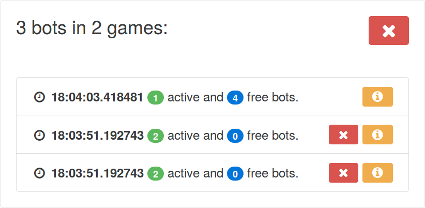
\includegraphics{assets/admin-games-list}
	\caption{Náhled seznamu her v administraci}
	\label{fig:admin-games-list}
\end{figure}

\begin{figure}[H]
	\centering
	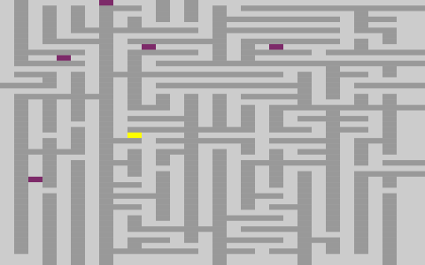
\includegraphics{assets/admin-game-detail}
	\caption{Náhled detailu hry v administraci}
	\label{fig:admin-game-detail}
\end{figure}

\begin{figure}[H]
	\centering
	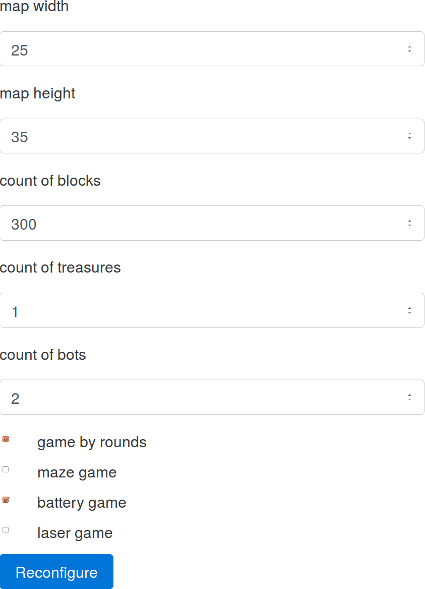
\includegraphics{assets/admin-conf-form}
	\caption{Náhled administračního formuláře pro konfiguraci}
	\label{fig:admin-conf-form}
\end{figure}

\section{Interní implementace aplikace}
\label{sec:implementation}

\subsection{Pomocná třída Exportable}

Abstraktní třída \ic*Exportable* je určena k identifikování všech tříd, jejichž instance je schopna se vyexportovat. Obsahuje jedinou metodu \ic|export|, která by v potomcích vracet jedině takové hednoty, které jsou zakódovat do formátu \nameref{subsec:json} - v naprosté většině případů se v aplikaci k exportu používá vestavěný datový typ \ic|dict|.

\subsection{Enumerace Orientation}

Tato enumerace dědící ze třídy \ic|IntEnum| z balíčku \ic|enum| zajištuje především sjednocení udávaných orientací v aplikaci, v některých případech označuje i směr. Je označena dekorátorem \ic|unique|, který zajištuje unikátnost jednotlivých hodnot v enumeraci. Tato enumerace obsahuje klíče \ic|NORTH|, \ic|EAST|, \ic|SOUTH| a \ic|WEST| s hodnotami v rozsahu od 1 do 4. Jako jednoduché utility jsou ve třídě metody (resp. vlastnosti díky dekorátoru \ic|@property|) \ic|is_horizontal| a \ic|is_vertical| ověřující horizontální, resp. vertikální směr. Výhoda v předkovi \ic|IntEnum|, resp. \ic|Enum| tkví v možnosti testovat shodnost pomocí operátoru rovnosti a konstruovat tyto objekty pomocí číselné hodnoty, viz následující ukázka.

\begin{lstlisting}[caption={Výhody třídy Enum}]
orientation_by_key = Orientation.NORTH
orientation_by_value = Orientation(0)

assert orientation_by_value == orientation_by_key
\end{lstlisting}

\subsection{Enumerace Action}

Enumerace \ic|Action| se v aplikaci používá jako jednoznačný identifikátor akce pro jednotlivé boty. Je stejně jako \ic|Orientation| odekorována pomocí \ic|@unique|, ale narozdíl od ní se nejedná o číselnou enumeraci, ale o enumeraci řetězců - pro snažší identifikaci v rámci požadavků na server.
Mezi její hodnoty patří \ic|STEP| pro pohyb robota, \ic|TURN_LEFT| a \ic|TURN_RIGHT| pro jeho otáčení, \ic|WAIT| pro čekání na místě (a nabití baterie) a \ic|LASER_BEAM| pro aktivaci laserového paprsku.

\subsection{Enumerace Field}

\todo{Enumerace Field a její klíče}

\subsection{Kontejnerová třída Map}

\ic|Map| je implementována jako dvourozměrná instance datového typu \ic|list|. Při inicializování objektu je ihned v konstruktoru (metoda \ic|__init__|) vytvořen dvourozměrný seznam - první rozměr pro výšku, druhý pro šířku. Oba tyto parametry jsou předány konstruktorem a je ověřena jejich nenulovost. Celý kontejner je naplněn instancemi třídy \ic|EmptyField|. Mezi další metody této třídy patří \ic|get_field_occurrences|, vracející seznam souřadnic, na kterých se nachází instance předáné třídy. Slouží k vyhledávání nad mapou, ale bohužel je její složitost vzhledem k implementaci $O(n^2)$. Metoda \ic|get_next_field| je určena k získávání vedlejší pole dle zadaných souřadnit a instance třídy \ic|Orientation|. V případě nemožnosti získat další pole ve směru na kraji mapy je vráceno \ic|None|. 

Níže uvedení příklad znázorňuje přetížené indexování instancí třídy \ic|Map| pomocí pozice uložené v vestavěném datovém typu \ic|tuple| (nebo jakýkoliv jiný objekt, který implementuje metodu \ic|__iter__|). Výsledkem je instance prázdného herního pole.

\begin{lstlisting}[caption={Přetížené indexování třídy Map}]
position = 3, 2
game_map = Map(width=10, height=10)

assert isinstance(
	game_map[position],
	EmptyField
)
\end{lstlisting}

\subsection{Třídy reprezentující herní bloky}

Na tomto místě je nutno poznamenat, že potomci třídy \ic|Field|, jenž jsou umisťováni do mapy, nejsou zodpovědni za své umístění, tzv. neuchovávají žádné informace o své pozici, ale pouze informace o svém stavu, jako jsou například orientace, jméno nebo stav baterie. 

\subsubsection{Společný abstraktní předek Field}

Pro všechny instance polí existuje společný abstraktní předek - třída \ic|Field|, ze které dědí všechna možná pole umístitelná do mapy. Samotná třída je potomkem třídy \ic|Exportable|, znamená to tedy, že každý z potomků této třídy musí implementovat metodu \ic|export|, což zajištuje možnost reprezentace herní struktury i mimo aplikaci.

\subsubsection{Prázdné pole EmptyField}

Jedná se o prázdnou variantu herního pole, je zodpovědná pouze za svůj korektní export.

\subsubsection{Pole bloku BlockField}

Třída \ic|BlockField| je ve své jednoduchosti velmi podobná prázdnému poli. Jediný rozdíl skrývá rozdílný přístup třídy \ic|Game| při herních akcích - na pole s objektem této třídy není možné vstoupit botem, avšak při zapnutém parametru pro laser hru je možno tento blok zničit. Po zničení je instance pole s blokem nahrazena instancí prázdného pole.

\subsubsection{Pole pro poklad TreasureField}

Ve své podstatě se jedná o pole jako každé jiné v mapě, avšak má jednu spicální vlastnost. Při vstoupení na něj botem je vyvolána výjimka \ic|GameFinished| (o struktuře a systému výjimek v sekci \fullref{subsec:custom-exceptions}) a hra končí. 

\subsubsection{Pole pro boty BotField a LaserBatteryBotField}

\subsection{Systém a struktura vlastních výjimek}
\label{subsec:custom-exceptions}

Proces zpracování herní akce je záležitost, při které může dojít až k několika desítkám nevalidních nebo hru ukončujících stavů, jako např. bot mimo herní mapu, pohyb bota, který není na řadě, požadavek na neznámého bota, požadavek na neznámou mapu, nesprávná herní akce pro kontext hry anebo hra s již zaplněnými poli pro boty. Proto je v aplikaci navržen systém výjimek, které jsou vyhazovány v momentech, kdy je již proces zpracování akce zahájen.

\begin{table}[H]
	\begin{tabularx}{\textwidth}{| l | X |}
		výjimka & její popis \\
		\hline
		asd & \lipsum[1] \\
	\end{tabularx}
	\caption{Seznam vlastních výjimek a jejich popis}
\end{table}

\section{Použité technologie}
\label{sec:used-technologies}

\subsection{Python}
\label{subsec:python}

\begin{figure}[H]
 \centering
 \includesvg[width=.8\textwidth]{assets/python-logo}
 \caption{Logo programovacího jazyka Python}
\end{figure}

\begin{sloppypar}
	Python je moderní interpretovaný programovací jazyk, který byl navržen v~roce 1991\cite{python-docs} nizozemským programátorem Guido van Rossumem. Nabízí rozličná programovací paradigma: imperativní, procedurální, funkcionální nebo objektově orientované, které jsem ve své práci použil nejčastěji.

	Python je vyvíjen jako open source projekt, jeho zdrojové kódy jsou tedy veřejné a je možné do nich přispět. Jeho výchozí implementace se nazývá \href{https://en.wikipedia.org/wiki/CPython}{CPython} dle jazyka C, ve kterém je implementována. Mezi další jeho alternativní implementace patří \href{https://cs.wikipedia.org/wiki/Jython}{Jython} naprogramovaný v~jazyce \href{https://cs.wikipedia.org/wiki/Java_%28programovac%C3%AD_jazyk%29}{Java} nebo \href{https://cs.wikipedia.org/wiki/IronPython}{IronPython} implementovaný v jazyce \href{https://cs.wikipedia.org/wiki/C_Sharp}{C\#} v prostředích \href{https://cs.wikipedia.org/wiki/.NET}{.NET} a \href{https://cs.wikipedia.org/wiki/Mono_%28platforma%29}{Mono}.

	Jednou z~velkých výhod Pythonu je jeho rozšiřitelnost. Oficiální portál pro rozšiřující balíčky \href{https://pypi.python.org/pypi}{PyPi} aktuálně nabízí okolo 74 tisíc knihoven. Kterýkoliv z~těchto balíčků je možno pomocí nástroje pip nainstalovat a používat. Jednou z~dalších možností, jak rozšířit jeho funkčnost, je naprogramovat si vlastní rozšíření v~jazyce C.

	Python je aktuálně vyvíjen ve dvou hlavních větvích; větvi Pythonu verze 2 a verze 3. Motivace pro vydání verze 3 byla především ve sjednocení práce s~řetězci (Python verze 2 rozlišoval řetězce ASCII\footnote{\href{https://cs.wikipedia.org/wiki/ASCII}{American Standard Code for Information Interchange} - kódová tabulka znaků z~anglické abecedy a některých dalších kódových znaků} znaků a řetězce Unicode\footnote{\href{https://cs.wikipedia.org/wiki/Unicode}{Unicode} je vylepšená norma pro reprezentaci znaků do více bytů.} znaků), celočíselného dělení a některých syntaktických vylepšení jazyka.
\end{sloppypar}

Poslední vydaná verze Pythonu je 3.5 a její hlavní výhodou je přidání podpory pro asynchronní volání funkcí a podpory pro typovost parametrů a návratových hodnot funkcí a metod. Jsem zastáncem inovativního a progresivního vývoje, takže celý tento \textbf{projekt} spoléhá na \textbf{spouštění v~Pythonu verze 3}.

\subsubsection{Jednotkové testování}
\label{subsubsec:unit-testing}

\begin{sloppypar}
	Jednotkové automatické testování je jeden z~způsobů, jak vývojáři ulehčit úpravu, vytváření i mazání částí zdrojových kódů. Jednotka testu je v~množina asercí (předpokladů), které kontrolují vývojářem vytvořené modelové situace nad zdrojovým kódem programu. Automatické testování je poté automatické spouštění testů např. po změně zdrojového kódu a určení, zda testy prošly korektně (aserce všech testů jsou pravdivé). Samotný test je však psán samotným vývojářem, což při testování může vytvářet klamný dojem \uv{bezchybnosti} zdrojového kódu aplikace, protože vývojář jakožto člověk, je bytost chybující a samotný kód testů může být napsat chybně a aserce jsou v~tu chvíli bezpředmětné, protože jsou např. vždy pravdivé a znehodnocují tím korektnost a správnost testů projektu.

	Python nabízí celou řadu nástrojů pro spouštění testů (\href{https://docs.python.org/3/library/unittest.html}{unittest}, \href{https://nose.readthedocs.org/en/latest/}{nose}, \href{http://pytest.org/latest/}{pytest}, \href{https://github.com/DRMacIver/hypothesis}{hypothesis} nebo \href{http://nestorsalceda.github.io/mamba/}{mamba}). V~projektu jsem se rozhodl použít balíček \ic|unittest|, vzhledem k~tomu, že je vestavěný v~Pythonu od verze 3 a není tedy nutné instalovat další závislost.

	Níže je uveden příklad třídy k~testování. Třída \ic|MathOperations| je určena k~základním matematickým operacím, pro názornost pro sčítání a dělení.
\end{sloppypar}

\begin{code}[caption={Příklad třídy $MathOperations$ k~testování}]
class MathOperations(object):
	@staticmethod
	def add(a, b):
		return a + b

	@staticmethod
	def divide(a, b):
		return a / b
\end{code}

\begin{sloppypar}
	Pomocí volání \ic|MathOperations.add(40, 2)| získáme \ic|42|, resp. při \ic|MathOperations.divide(36, 6)| je výsledkem \ic|6|. Ve své práci používám balíček pro testování \ic|unittest| dodávaný přímo s~programovacím jazykem Python. Jako hlavní nástroj pro jednotkové testování nabízí tento balíček třídu \ic|TestCase|, která obsahuje celou řadu metod pro testování asercí (\ic|assertEqual|, \ic|assertTrue|, \ic|assertEqual|, \ic|assertIn|, \ic|assertIs| nebo i komplexnější jako \ic|assertDictEqual|, \ic|assertRegex| nebo \ic|assertDictContainsSubset|) a potomky této třídy je potom možno automaticky spouštět a vyhodnocovat. Tyto předpoklady tedy zapíšeme jako metody do obalující třídy:
\end{sloppypar}

\begin{code}[caption={Základní TestCase pro třídu $MathOperations$}]
class TestMathOperations(TestCase):
	def test_add(self):
		self.assertEqual(
			MathOperations.add(40, 2),
			42
		)

	def test_div(self):
		self.assertEqual(
			MathOperations.div(36, 6),
			6
		)
\end{code}

V~případě spuštění a úspěšného otestování této třídy bude očekávaný výstup:

\begin{code}[language=sh,caption={Ukázka výstupu ze spuštění testů}]
###\mbox{\textdollar} python3 test.py
test_add (TestMathOperations) ... ok
test_div (TestMathOperations) ... ok

------------------------------------
Ran 2 tests in 38ms

OK
\end{code}


{\itshape
	Ve své aplikaci používám vlastní poděděnou třídu \ic|TestCase|, protože pro každé pokročilejší testování pohledů frameworku Flask je nutné mít správně nakonfigurovaný objekt pro \uv{vnější} přístup ke serveru, a také kvůli zobecnění některých častých operací v~mých testech - detaily ohledně testů jsou v~sekci\fullref{sec:implementation}.
}


Poté ale může dojít k~následující změně zdrojového k\'{o}du - vznikne požadavek na metodu \ic|MathOperations.add|, a to konkrétně na zvýšení počtu parametrů na tři. Ne ve všech případech se ovšem bude volat tato metoda i se třetím parametrem, musí být tedy zajištěna \textbf{zpětná kompatibilita}.

\begin{code}[caption={Vylepšená implementace metoda $MathOperations.add$}]
@staticmethod
def add(a, b, c=0):
	return a + b + c
\end{code}

Do metody testující sčítání je tedy nutné přidat aserci i pro tři parametry:

\begin{code}[caption={Testovací metoda pro vylepšenou $MathOperations.add$}]
def test_add(self):
	self.assertEqual(
		MathOperations.add(40, 2),
		42
	)
	self.assertEqual(
		MathOperations.add(10, 7, 3),
		20
	)
\end{code}

\begin{sloppypar}
	Tímto testem máme potvrzenou korektnost jak pro dvouparametrické volání, tak pro \uv{nové} tříparametrické volání. Podstata úprava zdrojového kódu tkví v~zachování předchozích asercí - je tak zajištěna zpětná kompatibilita. Jako další požadavek na metodu \ic|MathOperations.add| může typicky přijít přidání dalšího parametru, kdy je vhodné vzhledem k~aktuální implementaci metody \ic|add| tuto metodu přeimplementovat následovně:
\end{sloppypar}

\begin{code}[caption={Finální implementace metody $MathOperations.add$}]
@staticmethod
def add(*values):
	return sum(values)
\end{code}

\textit{
  Zápis $*values$ je velmi specifický pro jazyk Python. V~případě, že se jedná o~volání funkce/metody, je objekt $values$ rozexpandován do jednotlivých parametrů. Nezáleží přitom, kolik má volaná metoda/funkce předepsaných parametrů, takže i v~tomto případě může přijít $TypeError$. Jedinou podmínkou je možnost iterovat přes objekt $values$ (musí definovat interní metodu $\_\_init\_\_$). \\Druhý případ tohoto zápisu se může vyskytovat v~hlavičce funkce/metody, v~tomto případě znamená téměř pravý opak předchozího případu - předané parametry jsou použity pro vytvoření objektu $values$, jenž jako datový typ $tuple$ obsahuje všechny tyto parametry. 
}

K~testovacím asercím lze přidat i jednu komplexnější obsahující volání s~vyšším počtem parametrů:

\begin{code}[caption={Finální test pro metodu $MathOperations.add$}]
def test_add(self):
	...
	values = tuple(randint(0, 100) for _ in range(10))
	self.assertEqual(
		MathOperations.add(*values),
		sum(values)
	)

\end{code}

\subsection{Flask}
\label{subsec:flask}
\begin{wrapfigure}[18]{L}{.35\textwidth}
    \centering
    \includesvg[width=.35\textwidth]{assets/flask-logo}
    \caption{Logo webového frameworku Flask}
\end{wrapfigure}

Flask je webový framework implementovaný v~jazyce Python. Mezi jeho přednosti patří vestavěný vývojářský server, plná podpora pro unit testování a kvalitní dokumentace. Vzhledem k~jeho variabilitě a v~základu tenké architektuře bylo nutné přidat abstraktní vrstvy pro samotné zpracování herních akcí a podobně.

Vzhledem k~tomu, že je framework téměř stoprocentně pokryt testy, lze jednoduše usuzovat z~těchto testů o~funkčnostech frameworku a také je velmi snadné psát vlastní testy na kteroukoliv komponentu aplikace.

\subsection{HTTP}
\label{subsec:http}
\begin{sloppypar}
	HTTP (HyperText Transfer Protocol) je standardizovaný internetový protokol pro výměnu HTML kódu. Jeho první koncept vznikl v~roce 1991 jako veze 0.9, o~pět let později byla uvedena verze 1.1 a verze 1.1, která je používaná dodnes byla uvedena v~červu roku 1999. V~dnešní době je používán nejen k~výměně HTML kódu, ale jeho rozšíření MIME \footnote{Multipurpose Internet Mail Extensions} poskytuje možnost přenosu souborů jakéhokoliv typu. Samotný HTTP nezajištuje zabezpečení ani integritu dat. Nadstavbu nad HTTP tvoří HTTPS, jehož komunikace je šifrována pomocí SSL nebo TLS.

	HTTP pracuje na principu request-response (požadavek-odpověd). HTTP požadavek ve formě plaintextu je vyslán ze klientského zařízení, ten je serverem zpracován a nazpět jsou odeslány tzv. hlavičky odpovědi a poté i samotné její tělo. Vzhledem k~tomu, že každý další následující dotaz klienta na server bude nezávislý na těch předchozích, je nutno označit tento protokol za bezstavový. Nelze tedy uchovávat stav komunikace a jednotlivé požadavky nemají mezi sebou souvislost. Tato vlastnost může být částečně potlačena použitím HTTP tzv. sušenek (\emph{cookies}), které jsou schopny téměř jednoznačně identifikovat klientské zařízení na serveru.
\end{sloppypar}

\subsection{JSON}
\label{subsec:json}

JSON (\emph{JavaScript Object Notation}) je datový formát pro přenos dat nezávislý na platformě. Oproti jeho hlavnímu konkurentu XML\footnote{\href{https://cs.wikipedia.org/wiki/Extensible_Markup_Language}{Extensible Markup Language} je značkovací jazyk určený pro serializaci dat.} je datově úspornější, avšak je nevhodný k~přenosu binárních informací. JSON je schopen kódovat a následně dekódovat datové typy uvedené v~tabulce\fullref{table:json-types}.

\begin{figure}[H]
	\begin{minipage}{.6\textwidth}%
		\newcolumntype{B}{>{\bfseries}l}%
		\begin{tabular}{ B | p{6.5cm} }%
			typ & popis \\
			\hline
			integer & celočíselné hodnoty: $6$, $-3$ nebo $0$ \\
			float & desetinná čísla: $6.6$, $-3.5$ nebo $0.9$ \\
			string & řetězec znaků: $"bar"$ \\
			boolean & pravdivostní hodnoty $true$ a $false$ \\
			array & netypový seznam: $[6, 3.5, "foo"]$ \\
			object & objekt \textit{klíč} - \textit{hodnota}: \{"foo": 6, "bar": [1, 10, 100]\} \\
		\end{tabular}
		\captionof{table}{Seznam datových typů formátu JSON\label{table:json-types}}
	\end{minipage}%
	\hfill%
	\begin{minipage}{.3\textwidth}
	    \centering
	    \includesvg[width=\textwidth]{assets/json-logo}
	 	\captionof{figure}{Logo datového formátu JSON}%
	\end{minipage}
\end{figure}

\begin{code}[language=json,caption={Ukázka datového formátu JSON}]
{"map": [
	[
		1,
		{
			"field": 2,
			"orientation": 0,
			"your_bot": true
		}
	],
	[
		0,
		3
	]
	], "map_resolutions": "2x2"
}
\end{code}
\section{Použité metatechnologie}
\label{sec:used-metatechnologies}

\subsection{Git}
\label{subsec:git}

\begin{wrapfigure}{R}{.5\textwidth}
 \centering
 \includesvg[width=.5\textwidth]{assets/git-logo}
 \caption{Logo verzovacího systému Git}
\end{wrapfigure}

Git je distribuovaný systém správy verzí, původně určený pro vývoj jádra Linuxu. Jako jeho autor je označován Linus Torvalds\cite{git-docs}, jeho vznik se datuje kolem 2005 a v~roce 2016 je nadále aktivně vyvíjen; jeho poslední verze nese označení 2.7.3 a byla vydána 10. března 2016. Nejčastěji slouží k~verzování zdrojového kódu - vytváří historii pro každou část spravovaného repozitáře.

Repozitář je v~tomto systému základní nejvyšší jednotka pro správu zdrojového kódu, zapouzdřuje jednotlivé vývojové větvě, ve kterých může probíhat vývoj od jednotlivých vývojářů zcela odděleně. Git je oproti jiným verzovacím nástrojům velmi silný v~následném spojování těchto větví - v~případě nekonfliktních změn je toto spojení schopen provést zcela sám, v~případě těch konfliktních zvládne označit konfliktní místa - pro následné vyřešení konfliktů stačí vyřešit konflikty přímo ve zdrojových souborech, avšak existují i grafická rozhraní. Schéma základních operací je možno pochopit z~obrázku\fullref{fig:git-operations}.

\begin{figure}[H]
 	\centering
 	\includesvg[width=.9\textwidth]{assets/git-operations}
 	\caption[Základní operace při práci se systémem Git]{Základní operace při práci se systémem Git\cite{basic-git-svg}}
 	\label{fig:git-operations}
\end{figure}

Git je plně ovladatelný z~příkazové řádky, avšak existuje velké množství jeho grafických nadstaveb, například jednoduchý \href{http://git-cola.github.io/}{git-cola} (náhled v~obrázku\fullref{fig:git-cola}) nebo o~mnoho komplexnější \href{https://www.sourcetreeapp.com/}{SourceTree}.

\begin{figure}[H]
	\centering
	% \begin{minipage}{.475\textwidth}
 % 		\centering
 % 		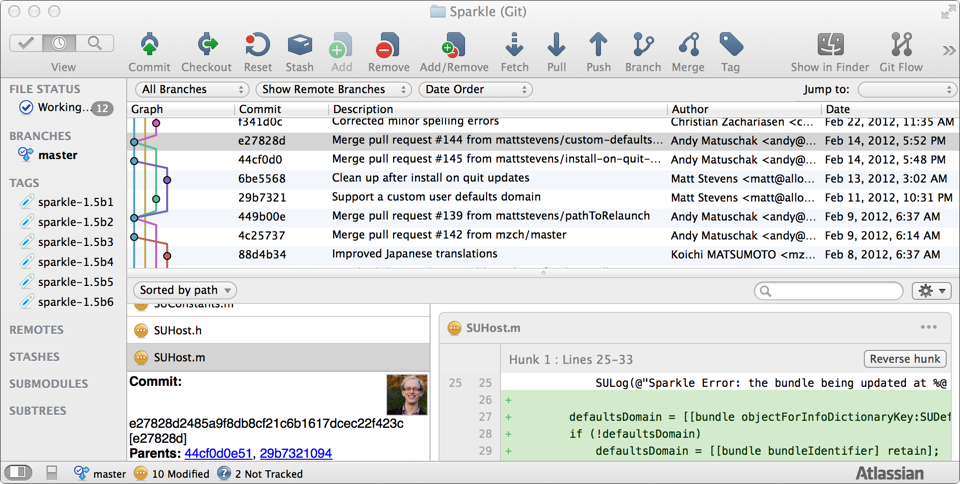
\includegraphics[width=\textwidth]{assets/source-tree-screenshot}
 % 		\caption{Screenshot z programu SourceTree}
	% \end{minipage}
	\begin{minipage}{.9\textwidth}
 		\centering
 		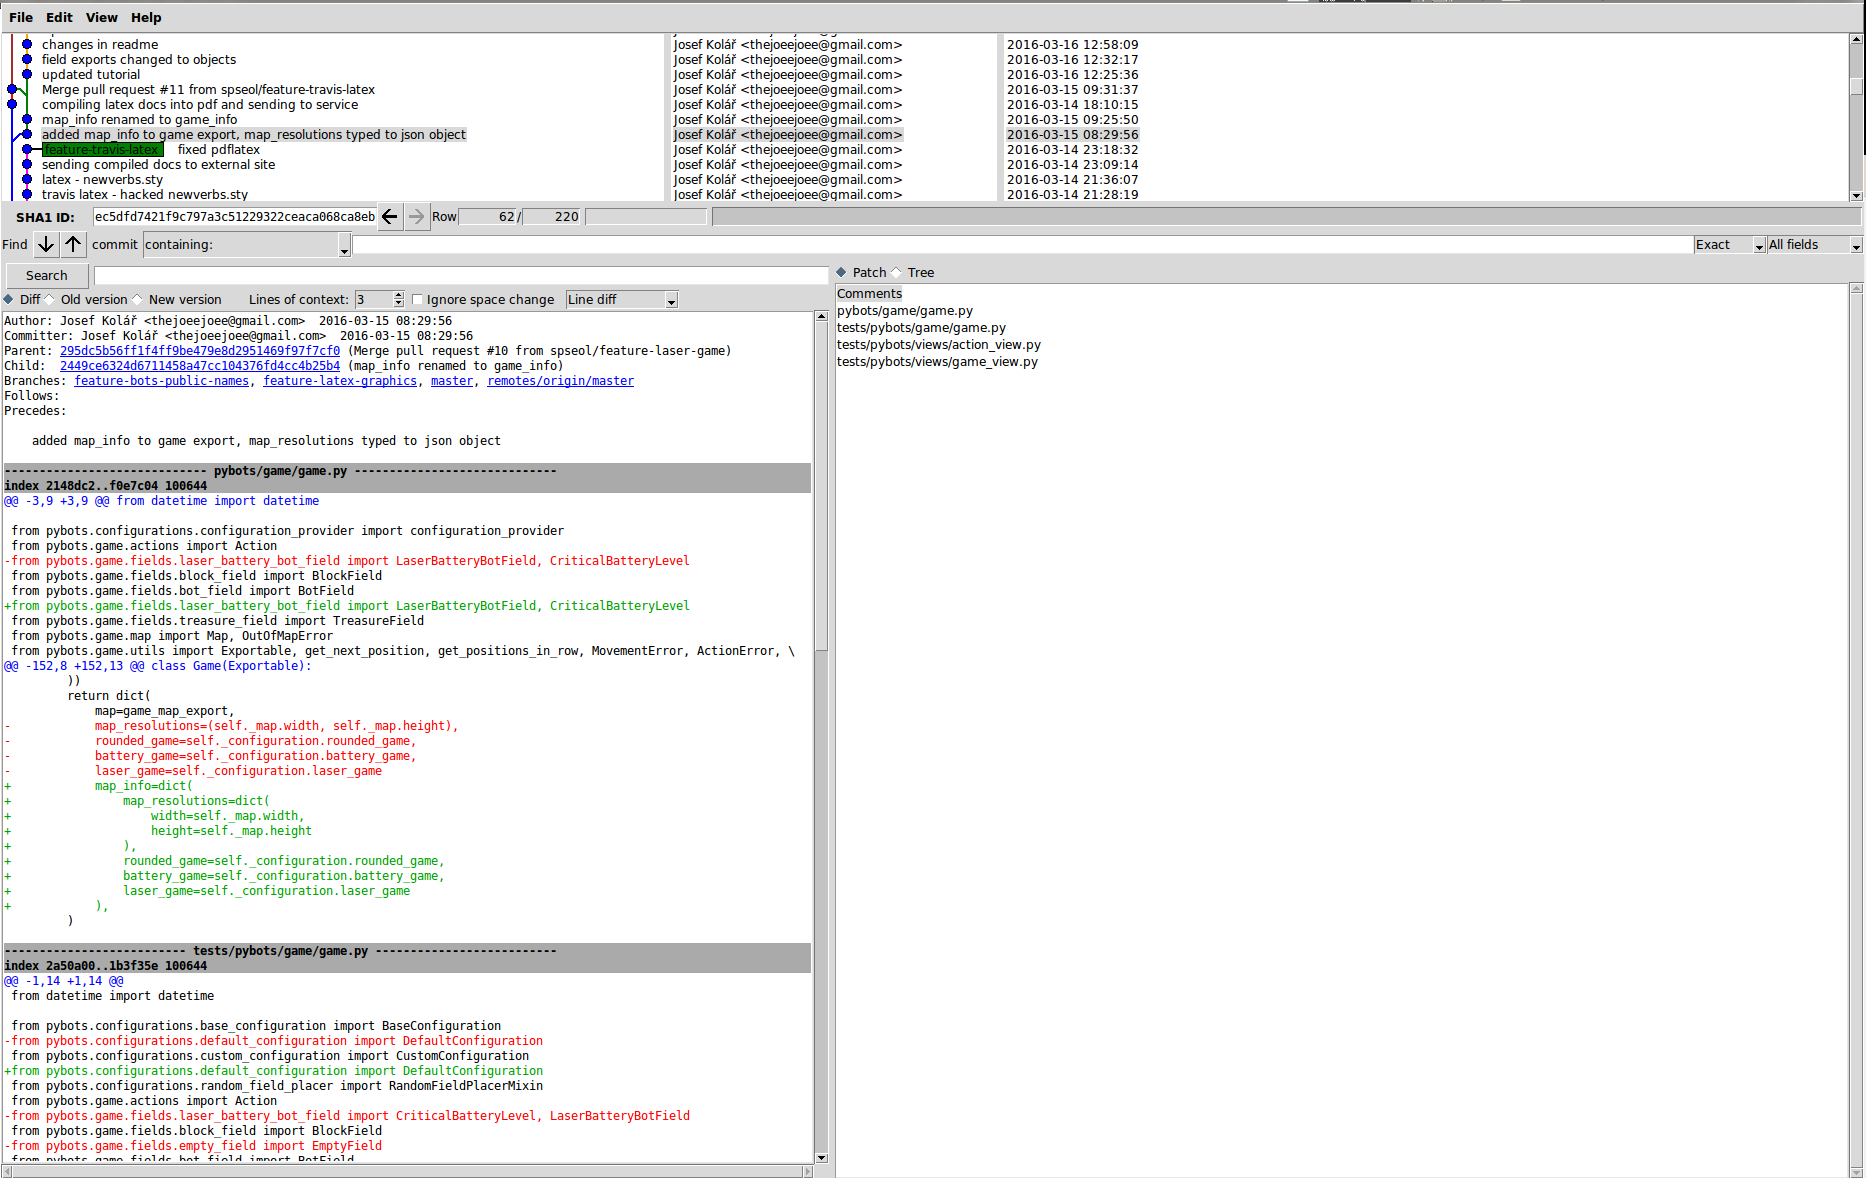
\includegraphics[width=.9\textwidth]{assets/git-cola-screenshot}
 		\caption{Screenshot z~programu git-cola}
 		\label{fig:git-cola}
 	\end{minipage}
\end{figure}

\subsection{GitHub}

\begin{wrapfigure}[18]{R}{.4\textwidth}
 	\centering
 	\includesvg[width=.4\textwidth]{assets/github-logo}
 	\caption{Logo systému pro správu git repozitářů GitHub}
\end{wrapfigure}

GitHub je webová služba poskytující podporu pro hostování \nameref{subsec:git} repozitářů. Pro veřejné repozitáře je tato služba zcela zdarma, pro soukromé repozitáře je zpoplatněna\cite{github-docs}. Kromě hostování nabízí i širokou škálu služeb týkajících se zdrojového kódu, jako například komentování zdrojového k\'{o}du, komentování jeho změn, systém úkolů, soukromých zpráv mezi vývojáři nebo možnost zařazení repozitáře mezi oblíbené. GitHub spustili v~roce 2008 vývojáři Tom Preston-Werner, Chris Wanstrath a PJ Hyett a nabízí i možnost napojení na jiné systémy, jako je například \nameref{subsec:travis-ci}. GitHub umí na základně uživatelských akcí (\ic|git push|, \ic|git pull|, \ic|git clone| a další) notifikovat externí služby pomocí HTTP POST požadavku na specifikovanou URL adresu - tato vlastnost se nazývá \uv{webhooks}. Repozitář tohoto projektu je také uložen na GitHubu pro adresou \url{https://github.com/spseol/pybots-server}.

\subsection{Travis CI}
\label{subsec:travis-ci}

Travis CI je webová služba zajišťující automatické sestavení a otestování změn zdrojového kódu v~repozitáři na GitHubu. Je řízen souborem \ic|.travis.yml|\cite{travis-docs}, ve kterém jsou definovány příkazy pro instalaci a nastavení prostředí a následné sestavení a spuštění testů projektu. Travis CI je specifický v~tom, že pro každé sestavení (\uv{build}) je rozběhnut samostatný kontejner s~nainstalovaným virtuální systémem. V~době psaní této práce je to distribuce \ic|Ubuntu 12.04.5 LTS|. 

\begin{wrapfigure}[16]{R}{.4\textwidth}
	\centering
	\includesvg[width=.4\textwidth]{assets/travis-logo}
	\caption{Logo automatického sestavovacího nástroje Travis CI}
\end{wrapfigure}

Při instalaci je možnost používat tradiční příkazy zapsané jazyce \ic|bash|, který tato distribuce používá jako výchozí příkazový interpret. \fullref{lst:travis-yml} také ukazuje možnost testovat projekt nad více verzemi Pythonu, v~mém případě je to \ic|Python 3.5.0|, \ic|Python 3.4.2|, \ic|PyPy 2.4.0 [Python 3.2.5]| (\href{http://pypy.org/}{interpret} Pythonu napsaný v~Pythonu) a \ic|nightly|, což je poslední vydaná verze Pythonu, aktuálně se jedná o~\ic|Python 3.6.0a0|. Detaily a historii sestavování jednotlivých změn zdrojového kódu lze zhlédnout na adrese \url{https://travis-ci.org/spseol/pybots-server}.

V~ukázce lze vidět také příkazy spouštěné při běhu kontejneru (\ic|install|, \ic|before_script|, \ic|script| a \ic|after_success|), ve kterých se postupně nejprve nainstalují Python závislosti ze souboru \ic|requirements.txt|, poté zaznamenávač pokrytí kódu \ic|coverage| a poté linter \ic|pep8|, který následně zkontroluje zdrojový kód a v~případě úspěchu se na řádku $17$ spustí samotné testy. Celý běh je zakončen odesláním výsledků pokrytí na službu \href{https://coveralls.io/}{coveralls.io}. V~sekcích \ic|language|, \ic|python| a \ic|matrix| je uložena konfigurace pro různé verze jazyka Python.

\begin{lstlisting}[caption={Zkrácená ukázka konfiguračního soubotu .travis.yml},label={lst:travis-yml},keywords={}]
language: python
python:
  - 3.4
  - 3.5
  - pypy3
  - nightly

install:
  - pip install -r requirements.txt
  - pip install coveralls pep8
before_script:
  - pep8 --ignore=E501,E731 pybots

script:
  - coverage run --source=pybots test.py

after_success:
  - coveralls

matrix:
  allow_failures:
    - python: pypy3
    - python: nightly
\end{lstlisting}

\subsection{Pycharm}

\begin{wrapfigure}{R}{.4\textwidth}
	\centering
	\includesvg[width=.4\textwidth]{assets/pycharm-logo}
	\caption{Logo vývojového prostředí Pycharm}
\end{wrapfigure}

\begin{sloppypar}
	Pycharm je světově uznávané a profesionální vývojové prostředí (IDE - \emph{Integrated Development Environment}) použité k~vývoji této aplikace. Je vyvíjeno českou společností \href{https://www.jetbrains.com/}{JetBrains}, která mj. nabízí studentům volné licence pro nekomerční použití. Pycharm nabízí velmi širkovou škálu služeb týkajících se vývoje v~Pythonu - od základních i pokročilých forem refaktoringu\footnote{Refaktoring je cílená úprava zdrojového kódu za účelem zvýšení jeho přehlednosti nebo výkonnosti.}, přes integraci verzovacích systémů, jako je například i \nameref{subsec:git}, podporu Python frameworků, pokročilé debuggovací nástroje až podpoře i jiný jazyků než Python, např. HTML, CSS, Javascript či i povrchově \LaTeX{}. Pokročilý Python debugger zabudovaný v Pycharmu je schopen pozastavit běh programu a nabídnout vývojáři možnost prohlédnout si hodnoty proměnných v aktuálním kontextu, procházet celý zásobník volání nebo provádět vlastní kód nad zvoleným kontextem v běžícím programu.
\end{sloppypar}

\subsection{\LaTeX}

\begin{wrapfigure}{R}{.5\textwidth}
	\centering
	\includesvg[width=.5\textwidth]{assets/latex-logo}
	\caption{Logo nástroje \LaTeX}
\end{wrapfigure}

K sazbě této práce byl použit balík \LaTeX, který obsahuje makra programu \TeX, který je nástrojem pro sazbu textu, především matematických vzorců a odborných publikací. Usnaďnuje především sázení obrázků, tabulek a další figur do textu, konfigurovatelné číslování nadpisů i generování obsahu, seznamu obrázků, tabuler, příloh i referencí.


\section{Závěr}

Podařilo se mi naprogramovat herní server v plném rozsahu zadání.
\todo{Zhodnotit a sepsat, jak je vše super}

\subsection{Možná budoucí vylepšení}

\begin{itemize}
 \item pro bezpečnější použití by bylo vhodné znovu navrhnout a vylepšit systém autorizace k přístupu k ovládání bota - \ic|bot_id| jakožto soukromý klíč přenášený po HTTP protokolu není nejbezpečnější metoda
 \item přidat herní log, ze kterého bude možné zrekonstruovat celý průběh hry od vygenerování až po vítězství jednoho z botů  
 \item do samotné hry je poměrně snadné přidat herní prvky, takže není problém přidat bonusové herní bloky, teleporty bloků, systém min nebo obranná elektromagnetická pole
\end{itemize}



\renewcommand\sectionbreak{}
\newpage

\listoftables
\addcontentsline{toc}{section}{Seznam tabulek}

\lstlistoflistings
\addcontentsline{toc}{section}{Seznam zdrojových kódů}

\listoffigures
\addcontentsline{toc}{section}{Seznam obrázků}

\renewcommand{\refname}{Seznam použitých zdrojů}
\newdateformat{bibciteformat}{\THEYEAR-\twodigit{\THEMONTH}-\twodigit{\THEDAY}}

\newcommand{\wwwbibitem}[3]{%
	#1. \textit{#2}. [online]. \bibciteformat\today\ [cit. \today].\\
	\emph{Dostupné z} \href{#3}{#3}%
}

\begin{thebibliography}{00}
	\bibitem{python-docs}
	\wwwbibitem{Python 3.5.1 documentation}{Python}{https://docs.python.org/3/}

	\bibitem{flask-docs}
	\wwwbibitem{Flask Documentation (0.10)}{Flask}{http://flask.pocoo.org/docs/0.10/}

	\bibitem{bootstrap-docs}
	\wwwbibitem{Bootstrap}{Bootstrap}{http://v4-alpha.getbootstrap.com/}

	\bibitem{fabric-docs}
	\wwwbibitem{JSDoc}{FabricJS}{http://fabricjs.com/docs/}

	\bibitem{jquery-docs}
	\wwwbibitem{jQuery API Documentation}{jQuery}{http://api.jquery.com/}

	\bibitem{font-awesome-docs}
	\wwwbibitem{Font Awesome, the iconic font and CSS toolkit}{Font Awesome}{http://fortawesome.github.io/Font-Awesome/}

	\bibitem{git-docs}
	\wwwbibitem{Git - Documentation}{Git}{https://git-scm.com/doc}

	\bibitem{github-docs}
	\wwwbibitem{GitHub Help}{GitHub}{https://help.github.com/}

	\bibitem{travis-docs}
	\wwwbibitem{Travis CI User Documentation}{Travis CI}{https://docs.travis-ci.com/}

	\bibitem{http-rfc}
	\wwwbibitem{Hypertext Transfer Protocol -- HTTP/1.1}{The Internet Society (1999)}{https://www.w3.org/Protocols/rfc2616/rfc2616.txt}

	\bibitem{json-docs}
	\wwwbibitem{JSON}{JSON}{http://www.json.org/}

	\bibitem{latex-docs}
	\wwwbibitem{Documentation}{Share\LaTeX, Online \LaTeX\ Editor}{https://www.sharelatex.com/learn/Main\_Page}

	\bibitem{latex-pro-pragmatiky}
	\wwwbibitem{\LaTeX\ pro pragmatiky}{\LaTeX\ pro pragmatiky}{http://www.nti.tul.cz/\textasciitilde{}satrapa/docs/latex/latex-pro-pragmatiky.pdf}

	\bibitem{basic-git-svg}
	\wwwbibitem{Základy Gitu}{Petr Viktorín, 2015}{https://raw.githubusercontent.com/pyvec/cheatsheets/master/basic-git/basic-git-cs.svg}
\end{thebibliography}

\addcontentsline{toc}{section}{Reference} 
\end{document}
